\section{The crystal form factor}\label{sec:10.1}

A dark-matter particle of \SI{10}{MeV} that crosses silicon can transfer up to \SI{53}{keV} of momentum and deposit up to \SI{35}{eV} (\cref{tab:1-kinematics}). Whether it leaves an electron--hole pair behind depends, for each pair $(\vect{q},\omega)$, on how strongly the filled bands respond at that momentum and energy. In the simplest description of the crystal, electrons that move independently in the potential of clamped nuclei, that response is a sum over transitions from one valence state to one conduction state, each weighted by the square of the density vertex of \cref{sec:3.2}. Experiments quote it as the \emph{crystal form factor} of Essig and collaborators~\cite{essig2016direct}, and nearly every projected or published limit on electron scattering in silicon and germanium rests on a table of it.

\subsection{The independent-particle structure factor}

Electron scattering through a mediator that couples to the electron number uses one row of the master formula, the density $n_e(\vect{q})$, with $\mathfrak{D}_{ee} = |\tilde V(\vect{q})|^2$ and all other entries zero (\cref{sec:8.2}). The spectrum per unit target mass is then \cref{eq:8.2-spectrum} with the dynamic structure factor of the electrons in place of the contraction, which is \cref{eq:A.8-rate}.

At the base point $\mathfrak{T}_0$ of the expansion hierarchy, \cref{eq:8.5-base}, the nuclei are clamped, the temperature is zero and the electrons are independent particles. The ground state is then a single Slater determinant $|0\rangle$ in which the four valence bands of silicon are filled with both spins and the conduction bands are empty. The one-electron states are Kohn--Sham states, and the conduction energies are raised by the scissor shift of \cref{sec:3.4}, which leaves the states themselves unchanged.

In the Bloch basis the density operator is \cref{eq:3.2-ne}. Acting on $|0\rangle$, a term $c^\dagger_{m,\vect{k}+\vect{q},s}c_{n\vect{k}s}$ vanishes if $n$ is a conduction band, since there is no electron to remove, and if $m$ is a valence band, since the state is already occupied, unless it is the state just emptied. That exception requires $\vect{k} + \vect{q} \equiv \vect{k}$, that is $\vect{q} = \vect{G}$, and it returns $|0\rangle$ itself with $\omega = 0$, the elastic Bragg term that no detector sees. For $\omega > 0$,
\begin{equation}
  n_e(\vect{q})|0\rangle = \sum_s\sum_{\vect{k}\in\mathrm{BZ}}\sum_{v,c}\rho_{cv}(\vect{k},\vect{q})\,|c,\vect{k}+\vect{q},s;\,v\vect{k}s\rangle ,
  \label{eq:D.29-pairs}
\end{equation}
where the ket is $|0\rangle$ with the electron moved from $v\vect{k}s$ to $c,\vect{k}+\vect{q},s$. These pair states are orthonormal, and their energies above the ground state are $\varepsilon_{c,\vect{k}+\vect{q}} - \varepsilon_{v\vect{k}}$, with $\vect{k} + \vect{q}$ folded into the first zone by the Umklapp vector $\vect{G}_{\mathrm{U}}$ of \cref{eq:3.2-rho}. Each pair appears once in \cref{eq:D.29-pairs}: at fixed $\vect{q}$ the hole $v\vect{k}s$ fixes the crystal momentum of the electron. Inserting \cref{eq:D.29-pairs} into \cref{eq:4.2-Sab} with $a = b = n_e$, the two spins give equal terms, and the sum over the $N$ crystal momenta of the zone becomes $\Vol\int_{\mathrm{BZ}}\dd^3k/(2\pi)^3$ with $\Vol = N\Omega$ (\cref{sec:3.1}). The volume cancels against the $1/\Vol$ in the definition of $S$, and
\begin{keyresult}[Independent-particle structure factor of a semiconductor]
\begin{equation}
  S^0(\vect{q},\omega) = 4\pi\sum_{v,c}\int_{\mathrm{BZ}}\frac{\dd^3k}{(2\pi)^3}\,\bigl|\rho_{cv}(\vect{k},\vect{q})\bigr|^2\,\delta\bigl(\omega - \varepsilon_{c,\vect{k}+\vect{q}} + \varepsilon_{v\vect{k}}\bigr) ,
  \label{eq:10.1-S0}
\end{equation}
for $\omega > 0$ at $T = 0$, with $v$ over the valence and $c$ over the conduction bands. The electron-recoil rate at $\mathfrak{T}_0$ is \cref{eq:8.2-spectrum} with $\mathfrak{D}_{ee} = \pi\sigmae\FDM(q)^2/\mu_{\chi e}^2$ (\cref{eq:1.4-Vsq}) and $S = S^0$.
\end{keyresult}
\noindent The factor $4\pi$ in $S^0$ is the $2\pi$ of \cref{eq:4.2-Sab} times 2 for spin. Each transition counts once, with the square of an amplitude of order one, and the rate is a sum of $|\rho_{cv}|^2$ over pairs, weighted by energy conservation. The same expression is $-2\Imag R^0_{\vect{0}\vect{0}}(\vect{q},\omega)$, the head of the independent-particle bubble \cref{eq:4.6-R0} at $T = 0$: in the bubble, a pair costs $\varepsilon_{c,\vect{k}+\vect{q}} - \varepsilon_{v\vect{k}}$ and its resonant denominator carries the imaginary part $-\pi\delta(\omega - \varepsilon_{c,\vect{k}+\vect{q}} + \varepsilon_{v\vect{k}})$. So the codes that compute dielectric functions compute $S^0$ along the way, and the screened response of \cref{sec:10.2} starts from the same object.

As in \cref{chap:3}, $S^0$ vanishes below the smallest pair energy $E_{\mathrm{min}}(\vect{q})$ of \cref{eq:3.3-Emin}, and a mass is kinematically allowed only where \cref{eq:3.3-allowed} holds. Its total weight is fixed by the closure relation \cref{eq:3.2-closure}, each valence state distributes a total weight of one over all bands at $\vect{k}+\vect{q}$, and only the part that lands in conduction bands counts. The zeroth moment is therefore at most $4\pi\cdot4/\Omega$, four valence bands of unit weight, a bound reached only when every transition leads into a conduction band. At small $q$ most of the weight stays in the same band and is lost to the rate; at large $q$ it spreads over conduction bands far above the gap.

Its energy-weighted sum is fixed as well. For a local one-electron potential, the double commutator of \cref{sec:4.3} taken for one electron gives $\sum_m(\varepsilon_{m,\vect{k}+\vect{q}} - \varepsilon_{n\vect{k}})|\rho_{mn}(\vect{k},\vect{q})|^2 = q^2/2m_e$ for every state $n\vect{k}$, the sum running over all bands $m$. The terms in which $m$ is another valence band are absent from \cref{eq:10.1-S0}, but summed over $\vect{k}$ they cancel: each transition at $-\vect{q}$ is the reverse of one at $\vect{q}$, so the valence--valence sum at $-\vect{q}$ is minus the sum at $\vect{q}$, while $S^0(\vect{q},\omega) = S^0(-\vect{q},\omega)$ in silicon makes the two sums equal, and a sum equal to its own negative vanishes. The first moment of \cref{eq:10.1-S0} is then $4\pi\cdot4\cdot\Omega^{-1}\cdot q^2/2m_e = \pi\nd_eq^2/m_e$ with $\nd_e = 8/\Omega$, the $f$-sum rule \cref{eq:4.3-fsum} for the valence electrons, since $\int_{\mathrm{BZ}}\dd^3k/(2\pi)^3 = 1/\Omega$. It is the standard test of a computed $S^0$, with the caveats of \cref{sec:4.3} for nonlocal potentials.

Note that $\vect{q}$ in \cref{eq:10.1-S0} is the physical momentum transfer and is never folded. The crystal momentum of the final electron is $\vect{k} + \vect{q}$ reduced to the first zone, but the vertex $\rho_{cv}$ depends on the whole $\vect{q}$ through the Umklapp vector that stays in the plane wave (\cref{eq:3.2-rho}), and so do $\vmin$ and $\FDM$ on the dark-matter side (\cref{sec:1.3}). Two momentum transfers that differ by a reciprocal-lattice vector reach the same pairs with different amplitudes and different kinematic weights.

The structure factor of a crystal depends on the direction of $\vect{q}$, and the full velocity kernel of \cref{eq:8.2-spectrum} gives a rate that changes as the Earth turns the crystal through the dark-matter wind, the daily modulation of \cref{sec:11.7}. For the time-averaged rate of a target whose orientation is not resolved, the literature replaces $S^0$ by its average $\bar S^0(q,\omega)$ over the directions of $\vect{q}$. The velocity and angular integrals then reduce to the mean inverse speed, \cref{eq:A.8-eta}. The rate takes the isotropic form \cref{eq:A.8-rateiso},
\begin{equation}
  \frac{\dd\mathcal{R}}{\dd\omega} = \frac{\rho_\chi\,\sigmae}{4\pi\,\mchi\,\rho_T\,\mu_{\chi e}^2}\int q\,\dd q\;\FDM(q)^2\,\eta\bigl(\vmin(q,\omega)\bigr)\,\bar S^0(q,\omega) .
  \label{eq:10.1-rateiso}
\end{equation}
\Cref{app:A.8} explains why this is not the same as averaging the directional rate over a day: a detector at fixed latitude does not sample all orientations equally.

\subsection{Form-factor normalizations}

Essig, Fernandez-Serra, Mardon, Soto, Volansky and Yu wrote the same rate per target, with the target information collected into a dimensionless function~\cite[Eqs.~(3.13) and (3.17)]{essig2016direct}. In our notation their crystal form factor is
\begin{equation}
  |f_{\mathrm{crys}}(q,\omega)|^2 = \frac{q^3\,\Omega}{4\pi\alpha\,m_e^2}\,\bar S^0(q,\omega) ,
  \label{eq:10.1-fcrys}
\end{equation}
which is \cref{eq:A.8-fcrys} at $\mathfrak{T}_0$. The factor $q^3/\alpha m_e^2$ is chosen so that $|f_{\mathrm{crys}}|^2$ is close to one where the rate is made. We substitute $\Omega\bar S^0 = 4\pi\alpha m_e^2|f_{\mathrm{crys}}|^2/q^3$ into \cref{eq:10.1-rateiso} and use $\rho_T\Omega = M_{\mathrm{cell}}$, the cell mass:
\begin{equation}
  \begin{aligned}
  \frac{\dd\mathcal{R}}{\dd\omega} &= \frac{\rho_\chi\,\sigmae\,\alpha\,m_e^2}{\mchi\,M_{\mathrm{cell}}\,\mu_{\chi e}^2} \\
  &\quad\times\int\frac{\dd q}{q^2}\,\eta\bigl(\vmin(q,\omega)\bigr)\,\FDM(q)^2\,|f_{\mathrm{crys}}(q,\omega)|^2 .
  \end{aligned}
  \label{eq:D.29-rate}
\end{equation}
Multiplying by $\omega$ turns $\dd q/q^2$ into $\dd\ln q\,(\omega/q)$ and the left side into $\dd\mathcal{R}/\dd\ln\omega$. Of the crystal, only the cell mass is left outside the form factor, because $|f_{\mathrm{crys}}|^2$ is defined per cell:
\begin{limitbox}[Crystal form-factor rate][lim:10.1a]
At independent-particle level, unscreened, at zero temperature and with clamped nuclei, the electron-recoil spectrum per unit target mass is
\begin{equation*}
  \begin{aligned}
  \frac{\dd\mathcal{R}}{\dd\ln\omega} &= \frac{\rho_\chi\,\sigmae\,\alpha\,m_e^2}{\mchi\,M_{\mathrm{cell}}\,\mu_{\chi e}^2} \\
  &\quad\times\int\dd\ln q\;\frac{\omega}{q}\,\eta\bigl(\vmin(q,\omega)\bigr)\,\FDM(q)^2\,|f_{\mathrm{crys}}(q,\omega)|^2 ,
  \end{aligned}
\end{equation*}
after Ref.~\cite[Eqs.~(3.13) and (3.17)]{essig2016direct}, divided by the target mass.
\par\smallskip
{\centering
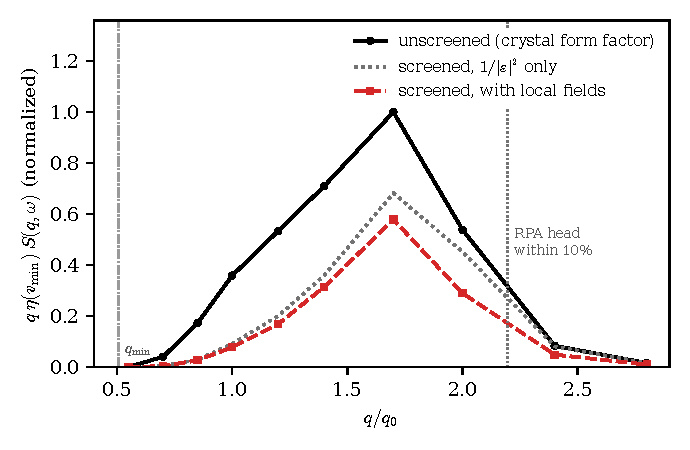
\includegraphics[width=\linewidth]{figures/ch10/limit10_1a.pdf}
\captionof{figure}{Unscreened rate against screened rates in silicon at $\omega = \SI{5}{eV}$, for $\mchi = \SI{10}{MeV}$ and a heavy mediator: the rate weight $q\,\eta(\vmin)\,S(q,\omega)$ of \cref{eq:10.1-rateiso} against $q$, normalized to the maximum of the unscreened curve. All three curves come from one model, the local empirical pseudopotential of \cref{we:8-lf-nuisance} (model gap \SI{0.82}{eV}), with $\vect{q}$ along the direction $(5,3,1)$, chosen so that no $\vect{q} + \vect{G}$ comes close to zero, and spectra averaged over 4.5 to \SI{5.5}{eV}. Solid: independent particles, the crystal form factor of the box. Dotted: random-phase screening by the macroscopic $1/|\varepsilon|^2$ alone, the leading correction. Dashed: random-phase screening with local fields over the 51 shortest reciprocal-lattice vectors, the fuller result. Dash-dotted: the smallest $q$ the halo reaches at \SI{5}{eV}. Dotted vertical: above $2.2\,q_0 = \SI{8.2}{keV}$, with $q_0 = \alpha m_e$, the macroscopic screening changes the rate by less than 10 percent. The model has no momentum components above $2.8\,q_0$, where the plot ends. Nothing is shaded. No $q$ in the plotted range brings the fuller result within 10 percent of the unscreened one.}\label{fig:10-fcrys-limit}
\par}
\smallskip
Near the kinematic edge the unscreened formula overstates the response twentyfold, at $q_0$ fourfold; macroscopic screening fades above about \SI{8}{keV}, but local fields keep the screened response near 0.6 of the unscreened one up to the largest $q$ this model can describe.
\end{limitbox}
\noindent The leading correction to the box lies on the many-body axis $\mathcal{X}$ of \cref{sec:8.5}: the polarization of the valence electrons screens the dark matter's potential and multiplies the response at small $q$ by roughly $1/|\varepsilon(q,\omega)|^2$, and the local fields of the crystal modify that factor. \Cref{sec:10.2} adds both. In silicon at \SI{5}{eV} the correction is not small (\cref{fig:10-fcrys-limit}). The kinematic edge at that energy lies at $0.525\,q_0$, with $q_0 = \alpha m_e = \SI{3.73}{keV}$; just above it, at $q = 0.55\,q_0$, screening cuts the response to 0.05 of the unscreened value, and at $q_0$ to 0.22. The local fields do not fade with $q$ as the macroscopic factor does: between 2 and $2.8\,q_0$ they hold the response at 0.54 to 0.61 of the unscreened value, with an uncertainty of about 10 percent from the size of the set of reciprocal-lattice vectors. Integrated over $q$, the screened rate at \SI{5}{eV} is 0.47 of the unscreened one. The model is cruder than the tabulated form factor, which it matches to within 25 percent at $q_0$, and \cref{sec:10.2} computes the same ratios from first-principles tables.

Written out with \cref{eq:10.1-S0}, $|f_{\mathrm{crys}}|^2$ is a double integral over the initial and final crystal momenta $\vect{k}$ and $\vect{k}'$ and a sum over the Umklapp vectors $\vect{G}'$ that connect them, the form in which Ref.~\cite[Eq.~(3.17)]{essig2016direct} defines it. For any function $g(\vect{q})$,
\begin{equation*}
  \int\frac{\dd^2\hat{\vect{q}}}{4\pi}\,g(q\hat{\vect{q}}) = \frac{1}{4\pi q^2}\int\dd^3q'\,\delta(q - |\vect{q}'|)\,g(\vect{q}') ,
\end{equation*}
since $\dd^3q' = q'^2\dd q'\,\dd^2\hat{\vect{q}}'$. At fixed $\vect{k}$, every $\vect{q}'$ is reached exactly once as $\vect{q}' = \vect{k}' - \vect{k} + \vect{G}'$ with $\vect{k}'$ in the first zone and $\vect{G}'$ a reciprocal-lattice vector, because the zones translated by all $\vect{G}'$ tile space. Then $\int\dd^3q' = \sum_{\vect{G}'}\int_{\mathrm{BZ}}\dd^3k'$, the final crystal momentum is $\vect{k}'$, and $\vect{G}'$ is the Umklapp vector of the transition. Applied to \cref{eq:10.1-S0},
\begin{equation*}
  \begin{aligned}
  \bar S^0(q,\omega) &= \frac{(2\pi)^3}{q^2}\sum_{v,c}\int_{\mathrm{BZ}}\frac{\dd^3k}{(2\pi)^3}\int_{\mathrm{BZ}}\frac{\dd^3k'}{(2\pi)^3}\sum_{\vect{G}'}\delta(q - |\vect{k}' - \vect{k} + \vect{G}'|) \\
  &\quad\times|\rho_{cv}(\vect{k},\vect{k}'-\vect{k}+\vect{G}')|^2\,\delta(\omega - \varepsilon_{c\vect{k}'} + \varepsilon_{v\vect{k}}) .
  \end{aligned}
\end{equation*}
Multiplying by $q^3\Omega/4\pi\alpha m_e^2$ and writing $(2\pi)^3/4\pi = 2\pi^2$,
\begin{equation}
  \begin{aligned}
  |f_{\mathrm{crys}}(q,\omega)|^2 &= \frac{2\pi^2}{\alpha m_e^2\Omega}\sum_{v,c}\int_{\mathrm{BZ}}\frac{\Omega\,\dd^3k}{(2\pi)^3}\int_{\mathrm{BZ}}\frac{\Omega\,\dd^3k'}{(2\pi)^3}\sum_{\vect{G}'}q\,\delta(q - |\vect{k}' - \vect{k} + \vect{G}'|) \\
  &\quad\times|\rho_{cv}(\vect{k},\vect{k}'-\vect{k}+\vect{G}')|^2\,\delta(\omega - \varepsilon_{c\vect{k}'} + \varepsilon_{v\vect{k}}) .
  \end{aligned}
  \label{eq:D.29-fcrys}
\end{equation}
Their prefactor $2\pi^2(\alpha m_e^2V_{\mathrm{cell}})^{-1}E_e^{-1}$ times their $E_e\,\delta(E_e - \cdots)$ is our $2\pi^2/\alpha m_e^2\Omega$ times the energy delta function, their $f_{[i\vect{k},i'\vect{k}',\vect{G}']}$ is $\rho_{cv}(\vect{k},\vect{k}'-\vect{k}+\vect{G}')$ in the plane-wave form \cref{eq:3.2-rhopw}, and the spin factor 2 sits in their $2\pi^2$ as it sits in our $4\pi$~\cite[Eq.~(A.29)]{essig2016direct}. The prefactor $2\pi^2/\alpha m_e^2\Omega$ is \SI{1.99}{eV} for silicon, with $\Omega = \SI{40.05}{\angstrom^3}$.

Since a tabulated form factor is used far from the paper that produced it, its normalization is where errors enter. The literature states the same rate in several normalizations, and each converts to $\bar S^0$ in one line.
\begin{itemize}
\item \emph{Structure factor, form factor and dielectric function.} $\Omega\bar S^0 = 4\pi\alpha m_e^2|f_{\mathrm{crys}}|^2/q^3$ and $|f_{\mathrm{crys}}|^2 = q^5\Omega\,\varepsilon_2/8\pi^2\alpha^2m_e^2$, \cref{eq:A.8-fcrys}; the second uses the unscreened $\varepsilon_2 = 2\pi\alpha\bar S^0/q^2$ of \cref{eq:A.7-SL} at $T = 0$, and agrees with Ref.~\cite[Eq.~(16)]{knapen2021dark}.
\item \emph{Per target or per unit mass.} A rate for a target of $N_{\mathrm{cell}}$ cells~\cites[Eq.~(3.13)]{essig2016direct}[Eq.~(36)]{catena2021crystal} is $N_{\mathrm{cell}}M_{\mathrm{cell}}$ times \cref{eq:D.29-rate}.
\item \emph{Sums over states.} Ref.~\cite[Eqs.~(3.6) and (3.12)]{griffin2021extended} writes the rate with the transition form factor $f_{i\to f}(\vect{q}) = \langle f|\ee^{\ii\vect{q}\cdot\vect{r}}|i\rangle$ between unit-normalized spatial orbitals and a separate spin factor. Then $(2\pi/\Vol)\sum_{i,f}|f_{i\to f}|^2\delta(\omega - E_f + E_i) = S^0/2$. The transition matrix element of the density in Ref.~\cite[Eqs.~(11) and (17)]{trickle2023exceed} is the vertex $\rho_{cv}(\vect{k},\vect{q})$ of \cref{eq:3.2-rho}.
\item \emph{Crystal-momentum weights.} Plane-wave codes replace $\int_{\mathrm{BZ}}\Omega\,\dd^3k/(2\pi)^3$ by $\frac12\sum_{\vect{k}}w_{\vect{k}}$ with weights that sum to 2~\cite[Eq.~(4.2)]{essig2016direct}. The 2 is the spin factor already present in the prefactor, and it must not be counted twice.
\item \emph{Bins.} A tabulated form factor is an average over bins of width $\Delta q$ and $\Delta\omega$~\cite[Eq.~(4.1)]{essig2016direct}, and \cref{eq:D.29-rate} becomes a double sum with $\dd q\,\dd\omega \to \Delta q\,\Delta\omega$. A table that stores the sum over a bin rather than the average differs by the bin widths.
\end{itemize}
A factor of two or ten in a rate is easy to make in these steps and hard to see in a plot. The $f$-sum rule catches it: at $q \approx q_0$, where the free recoil energy $q^2/2m_e = \SI{13.6}{eV}$ lies well inside the tabulated range, $\int\dd\omega\,\omega\,\bar S^0$ must come within some ten percent of $\pi\nd_eq^2/m_e$. A rigid scissor shift $\Delta_{\mathrm{scis}}$ raises it by $\Delta_{\mathrm{scis}}\int\dd\omega\,\bar S^0$, since it moves the weight without changing the vertices.

\subsection{The silicon form factor}

\Cref{fig:10-fcrys} shows the crystal form factor of silicon as Ref.~\cite{essig2016direct} tabulated it, from PBE bands with the gap set by a scissor shift, four valence and 52 conduction bands, and a plane-wave cutoff of \SI{70}{Ry}~\cite[Sects.~4.1 and 4.2]{essig2016direct}. The scissor puts the gap at \SI{1.11}{eV}, close to the room-temperature gap of \SI{1.12}{eV} (\cref{sec:10.7-edge}); the gap at zero temperature is \SI{1.17}{eV} (\cref{sec:3.3}), and a cryogenic detector sees the difference as a shift of the onset. The table begins at \SI{1.2}{eV}, its first bin above the gap, and ends at \SI{50}{eV}, where the highest conduction band runs out.
\begin{figure}[t]
  \centering
  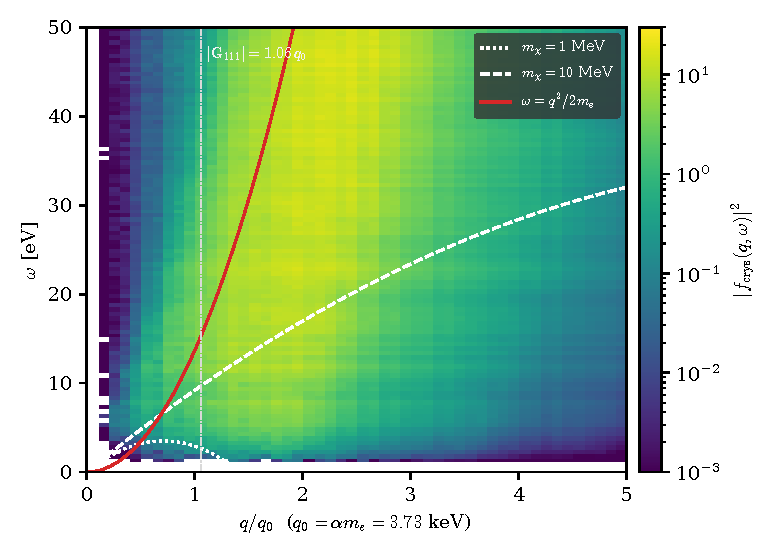
\includegraphics[width=0.85\linewidth]{figures/ch10/fig10_1.pdf}
  \caption{Crystal form factor $|f_{\mathrm{crys}}(q,\omega)|^2$ of silicon, \cref{eq:10.1-fcrys}, from the tabulation of Ref.~\cite{essig2016direct}: PBE bands with the gap set to \SI{1.11}{eV} by a scissor shift, valence to conduction, unscreened, averaged over the directions of $\vect{q}$. For display, bins are merged to $0.1\,q_0$ in $q$ and \SI{0.5}{eV} in $\omega$; white cells below $0.3\,q_0$ are bins that the grid of crystal momenta of the calculation does not reach, and white cells in the lowest row are bins next to the gap that hold no weight. White curves: the largest energy that dark matter of 1 and \SI{10}{MeV} can deposit at each $q$, $qv_{\mathrm{max}} - q^2/2\mchi$ with $v_{\mathrm{max}} = \SI{794.5}{km.s^{-1}}$ (\cref{eq:1.3-region}); everything below a curve is kinematically allowed. Red: the free-electron recoil $\omega = q^2/2m_e$, along which the weight concentrates at large $q$. Dash-dotted: $|\vect{G}_{111}| = \sqrt3\,2\pi/a = 1.06\,q_0$, the shortest reciprocal-lattice vector. The color scale is logarithmic.}\label{fig:10-fcrys}
\end{figure}

Divided by $\pi\nd_eq^2/m_e$ with the valence density $\nd_e = 8/\Omega$, the first moment of the tabulated $\bar S^0$ over its \SI{50}{eV} is 1.03 at $q_0$, and 1.1 to 1.2 between $0.3\,q_0$ and $0.7\,q_0$, as means over windows of $0.2\,q_0$ with the bins the grid does not reach counted as zero. The scissor shift raises the first moment, since it moves every transition up by about \SI{0.55}{eV} without changing its weight; that is the difference between the PBE gap of silicon (\cref{sec:3.4}) and \SI{1.11}{eV}. At small $q$, where the mean energy deposited is a few eV, the shift accounts for about ten percent; the rest of the excess has no identified cause (\cref{sec:10.10-manybody}). Beyond $1.5\,q_0$ the ratio falls, to 0.83 at $1.5\,q_0$ and 0.33 at $2\,q_0$: the free recoil energy is then 31 and \SI{54}{eV}, and the weight has moved past the last tabulated band. As a second check, the tabulated $\bar S^0$ at $q_0$ lies within 25 percent of the independent-particle structure factor of the local empirical pseudopotential of \cref{we:8-lf-nuisance}, along $[100]$, between 5 and \SI{20}{eV}. The two calculations share no input other than the crystal structure.

The form factor varies with $q$ on two scales that silicon happens to have in common, the zone scale and $q_0$ (\cref{sec:1.3}). At momentum transfers small compared with the zone, $2\pi/a = 0.61\,q_0$, the vertex reduces to its optical limit, $\rho_{cv} \simeq \vect{q}\cdot\vect{v}_{cv}/(\varepsilon_{c\vect{k}} - \varepsilon_{v\vect{k}})$ (\cref{sec:3.2}), so $\bar S^0 \propto q^2$ at fixed $\omega$, and by \cref{eq:A.8-fcrys} $|f_{\mathrm{crys}}|^2 \simeq q^5\Omega\varepsilon_2(\omega)/8\pi^2\alpha^2m_e^2$ with the optical $\varepsilon_2$. Integrated over energy, the tabulated form factor grows as $q^{4.8}$ between $0.3\,q_0$ and $0.75\,q_0$, close to this dipole scaling even where $q$ is no longer small compared with the zone. Near $|\vect{G}_{111}| = 1.06\,q_0$ the momentum transfer resolves the bond, the optical limit fails, and the vertex is set by the plane-wave content of the valence states at momenta of order $q$ (\cref{eq:3.2-rhopw}). At fixed $\omega$ between 3 and \SI{10}{eV}, $|f_{\mathrm{crys}}|^2$ peaks at $1.7$ to $1.8\,q_0$ and at $2\,q_0$ it is still 2.1 to 2.5 times its value at $q_0$; by $3\,q_0$ it has fallen to a quarter of its value at $q_0$. The factor $q^3$ in \cref{eq:10.1-fcrys} pushes this peak outward. The rate weight of \cref{eq:10.1-rateiso}, $q\bar S^0$, peaks earlier, at 1.1 to $1.4\,q_0$.

At large $q$ the figure shows where the weight goes. Along the red curve, $\omega = q^2/2m_e$, a dark-matter particle would give a free electron at rest its recoil energy, and at large $q$ the response of bound electrons gathers around it, broadened by their momenta, as in the impulse approximation of \cref{we:4-gas}. At a fixed small energy deposited, a large $q$ needs an electron that already moves against the momentum transfer with a momentum of about $q/2$, and the bound valence states have little weight at momenta much above $q_0$. That is why, integrated over the tabulated energies, $|f_{\mathrm{crys}}|^2$ falls as $q^{-5}$ between 2 and $4\,q_0$. The white curves show which part of the plane the halo can reach. Dark matter of \SI{1}{MeV} reaches only a thin sliver above the gap at $q < 1.4\,q_0$, near the bottom of the figure; at \SI{10}{MeV} it reaches deposits up to \SI{35}{eV} and momentum transfers well past the peak of $|f_{\mathrm{crys}}|^2$.

\begin{workedexample}{The silicon rate at \SI{10}{MeV}}\label{we:10-rate}
Take $\mchi = \SI{10}{MeV}$, $\sigmae = \SI{e-37}{cm^2}$ and the standard halo of \cref{app:A.8}: $\rho_\chi = \SI{0.3}{GeV.cm^{-3}}$, $v_0 = \SI{238}{km.s^{-1}}$, $v_{\mathrm{esc}} = \SI{544}{km.s^{-1}}$ and $v_{\mathrm{E}}^{\mathrm{ref}} = \SI{250.5}{km.s^{-1}}$. The reduced mass is $\mu_{\chi e} = \SI{486.2}{keV}$, so $m_e^2/\mu_{\chi e}^2 = 1.105$, and the number density is $\rho_\chi/\mchi = \SI{30}{cm^{-3}}$. The prefactor of the box, with $M_{\mathrm{cell}} = \SI{52.33}{GeV}$, is
\begin{equation*}
  \frac{\rho_\chi\,\sigmae\,\alpha\,m_e^2}{\mchi\,M_{\mathrm{cell}}\,\mu_{\chi e}^2}
  = \frac{\SI{30}{cm^{-3}}\times\SI{e-37}{cm^2}\times c\times1.105}{137.036\times M_{\mathrm{cell}}}
  = \SI{2.45e5}{kg^{-1}.yr^{-1}} ,
\end{equation*}
where the factor $c$ turns $\rho_\chi\sigmae/\mchi$ into a rate and $\eta$ is then a pure number, $\langle1/v\rangle = 1041$ in units of $1/c$. Everything else is the double integral of $\eta\FDM^2|f_{\mathrm{crys}}|^2\,\dd q\,\dd\omega/q^2$ over the tabulated bins, with $\vmin = \omega/q + q/2\mchi$ and $\eta$ in the closed form of \cref{app:D.1}.

For a heavy mediator, $\FDM = 1$, the double integral is 0.652, and the rate above the gap is
\begin{equation*}
  \mathcal{R} = \SI{2.45e5}{kg^{-1}.yr^{-1}}\times0.652 = \SI{1.60e5}{kg^{-1}.yr^{-1}} ,
\end{equation*}
about 440 events per kilogram and day. The spectrum $\dd\mathcal{R}/\dd\omega$ peaks at \SI{6.5}{eV}, its mean is \SI{6.0}{eV}, 38 percent of the events deposit at most \SI{4.9}{eV}, and it ends at \SI{35}{eV}, the largest energy a particle at $v_{\mathrm{max}}$ can deposit. At the peak energy the integrand in $q$ is flat between about $1.7\,q_0$ and $1.9\,q_0$ (6.5 to \SI{7.09}{keV}); only 5 percent of the rate comes from $q < q_0$, and 27 percent from $q > 2\,q_0$.

For a light mediator, $\FDM = (q_0/q)^2$, the integral is 0.193, and $\mathcal{R} = \SI{4.73e4}{kg^{-1}.yr^{-1}}$, about 130 per kilogram and day. The factor $(q_0/q)^4$ moves the rate to small $q$ and low energy: the spectrum peaks at \SI{3.3}{eV}, its mean is \SI{4.5}{eV}, 66 percent of the events deposit at most \SI{4.9}{eV}, and the $q$ integrand at the peak is largest near $0.6\,q_0 = \SI{2.2}{keV}$, near the kinematic edge. Now 44 percent of the rate comes from $q < q_0$.

The two mediators probe different parts of \cref{fig:10-fcrys}. The heavy mediator samples the form factor near its maximum, at twice $q_0$ and a few eV, where the bands and the plane-wave content of the valence states set the answer. The light mediator samples its small-$q$ edge, where the form factor is smallest and where, as the limit check shows, screening matters most. The scaling of \cref{eq:1.5-heuristic} gives the rest: at fixed $\sigmae$ the rate falls as $1/\mchi$ once $\mchi$ is well above the threshold and the reach in $q$ covers the peak. Published rates differ from these numbers mainly through the halo: Ref.~\cite{essig2016direct} uses $\rho_\chi = \SI{0.4}{GeV.cm^{-3}}$, $v_0 = \SI{230}{km.s^{-1}}$, $v_{\mathrm{esc}} = \SI{600}{km.s^{-1}}$ and an Earth speed of \SI{240}{km.s^{-1}}~\cite[Sect.~6]{essig2016direct}.
\end{workedexample}

\subsection{Convergence parameters and omitted physics}

A crystal form factor is computed from Kohn--Sham bands and plane-wave vertices. The bands come from a density-functional calculation with a pseudopotential (\cref{sec:3.4,sec:3.5}), with the gap set by a scissor shift or by quasiparticle corrections (\cref{app:E.1,app:E.3}). The vertex is the plane-wave overlap \cref{eq:3.2-rhopw}, evaluated for every valence state, every conduction state and every Umklapp vector that a given $\vect{q}$ requires, with $\vect{q}$ kept unfolded. \Cref{app:E.7} sets out the calculation and its cost, about $5\times10^{11}$ vertices for silicon with 52 conduction bands and momentum transfers up to \SI{30}{keV}. The plane-wave cutoff limits the largest $q$ a vertex can carry, the number of conduction bands the largest $\omega$, and the grid of crystal momenta the resolution at small $q$ and near the onset; the white cells of \cref{fig:10-fcrys} are this last limit. At large $q$ the pseudopotential matters as well. A pseudo-wavefunction is smooth inside the core region by construction, and above a few $q_0$ the vertex needs the nodes of the true valence states near the nucleus. The all-electron reconstruction of \cref{app:E.2} restores them; Griffin and collaborators found that it raises the valence-to-conduction rate of germanium at energies above about \SI{15}{eV}~\cite[Sect.~1]{griffin2021extended}. For silicon at \SI{10}{MeV}, \cref{we:10-rate} draws a quarter of the heavy-mediator rate from $q > 2\,q_0$, and that part rests on the same correction.

Its place in the expansion hierarchy, $\mathfrak{T}_0$, fixes what the calculation leaves out. It has no screening: the dark matter's potential acts on independent electrons, while in the crystal the other electrons polarize and reduce it, most strongly at small $q$, where the light mediator and the lightest masses collect their rate. \Cref{sec:10.2} adds the random-phase screening and the local fields, and shows when the loss function gives the rate exactly. It has no electron--hole attraction: an exciton moves weight from the continuum toward the gap, which matters for the lowest thresholds, and \cref{sec:10.5} treats excitons at finite momentum. It has no lattice: the nuclei are clamped, so the phonon-assisted transitions that open the indirect gap below the zero-phonon edge (\cref{sec:13.1}) and the Migdal effect (\cref{chap:12}) are absent. It holds only valence-to-conduction transitions: the $2p$ shell of silicon, \SI{99}{eV} below the valence maximum, and the $3d$ shell of germanium, about \SI{29}{eV} below it, are the subject of \cref{sec:10.6}, and the table ends at the highest conduction band it includes. And it is an angle average at zero temperature, which drops the daily modulation and the thermal shift of the gap.
